\documentclass[10pt,border=2pt]{standalone}
\usepackage{mathptmx}
\usepackage{amsmath,amssymb}
\usepackage{tikz}
\usetikzlibrary{positioning,arrows.meta}
\begin{document}
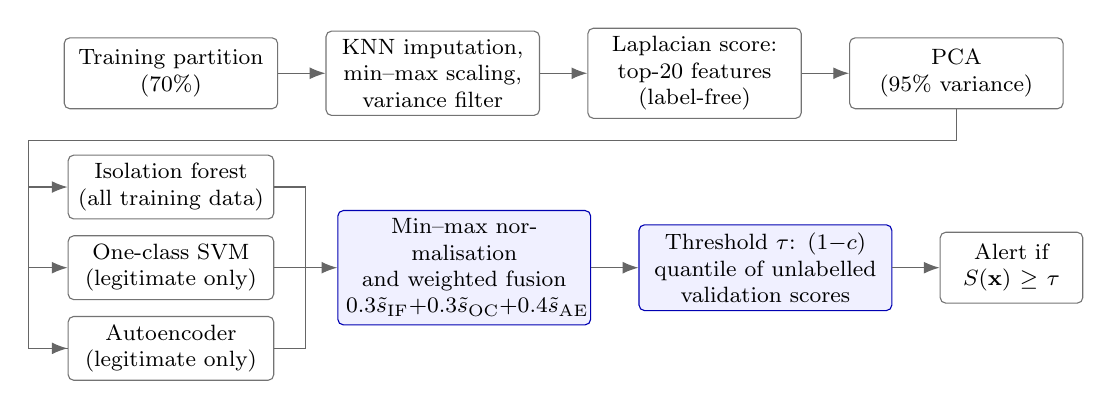
\begin{tikzpicture}[
  font=\footnotesize,
  box/.style={draw=black!55, rounded corners=2pt, align=center, minimum height=9mm, inner sep=3pt, text width=25mm},
  det/.style={box, text width=24mm, minimum height=7mm},
  acc/.style={box, draw=blue!70!black, fill=blue!6, text width=30mm},
  arr/.style={-{Latex[length=2mm]}, black!60}]
\node[box] (data) {Training partition\\(70\%)};
\node[box, right=6mm of data] (pre) {KNN imputation,\\min--max scaling,\\variance filter};
\node[box, right=6mm of pre] (fs) {Laplacian score:\\top-20 features\\(label-free)};
\node[box, right=6mm of fs] (pca) {PCA\\(95\% variance)};
\node[det, below=16mm of data] (oc) {One-class SVM\\(legitimate only)};
\node[det, above=2mm of oc] (if) {Isolation forest\\(all training data)};
\node[det, below=2mm of oc] (ae) {Autoencoder\\(legitimate only)};
\node[acc, right=8mm of oc] (fuse) {Min--max normalisation\\and weighted fusion\\$0.3\tilde s_{\mathrm{IF}}{+}0.3\tilde s_{\mathrm{OC}}{+}0.4\tilde s_{\mathrm{AE}}$};
\node[acc, right=6mm of fuse] (thr) {Threshold $\tau$: $(1{-}c)$\\quantile of unlabelled\\validation scores};
\node[box, right=6mm of thr, text width=16mm] (out) {Alert if\\$S(\mathbf{x})\ge\tau$};
\draw[arr] (data) -- (pre); \draw[arr] (pre) -- (fs); \draw[arr] (fs) -- (pca);
\coordinate (bus) at ([xshift=-5mm]if.west);
\draw[black!60] (pca.south) -- ++(0,-4mm) -| (bus);
\draw[black!60] (bus) |- (ae.west);
\draw[arr] (bus) -- (if.west); \draw[arr] (bus |- oc.west) -- (oc.west); \draw[arr] (bus |- ae.west) -- (ae.west);
\coordinate (mrg) at ([xshift=4mm]oc.east);
\draw[black!60] (if.east) -| (mrg); \draw[black!60] (ae.east) -| (mrg);
\draw[arr] (oc.east) -- (fuse.west);
\draw[arr] (fuse) -- (thr); \draw[arr] (thr) -- (out);
\end{tikzpicture}
\end{document}
